\newpage
\section{Ergebnisse}
\label{sec:ergebnisse}
Die Umrechnung des gemessenen Brechungsindexes in die Anteile an Ethanol und Cyclohexan, erfolgt anhand der gegeben Kalibrierung. Aus den Kalibrierdaten wird dazu eine polynomische Regressionsfunktion zweiten Grades ermittelt, anhand welcher sich durch Einsetzen der Werte für den Brechungsindex, der Anteil an Ethanol berechnen lässt. Eine Beispielrechnung dazu ist als Gleichung \eqref{gl:bsprechAnteil} nachfolgend aufgeführt. Die Berechnungsergebnisse sind in der Tabelle auf dem Vordruck eingetragen. Die Berechnung des Anteils des zweiten Stoffes Cyclohexan ist anhand der Gleichung \eqref{gl:anteilcyclo} nachzuvollziehen. 

\begin{figure}[h!]
	\begin{center}
		%\resizebox{0.8\textwidth}{!}{
		\begin{tikzpicture}[trim axis left, trim axis right]
		\begin{axis}[
		axis lines = left,
		width = 13cm,
		height = 7cm,
		xmin = 0,
		xmax = 1.05,
		ymin = 1.3,
		ymax = 1.47,
		ytick = {1.3,1.35,...,1.5},
		xtick = {0,0.1,...,1.1},
		ylabel={Brechungsindex},
		y label style={at={(-0.03,0.5)}},
		xlabel={x(Ethanol)},
		legend style={at={(0.1,0.95)},anchor=west}
		]
		\addplot table {kalibrierpunkte.dat};
		
		\addplot +[mark=none, dashed, black, domain=0:1.1] {-0.0262541672*x^2-0.0374560519*x+1.4232079871};
		\legend{Messpunkte der Kalibrierung,Kalibrierfunktion mit R$^2$=\SI{0,999}{} (\ref{gl:Regressionsgeradengleichung})};
		\end{axis}
		\end{tikzpicture}
		%	}Ventilkennlinie
		\caption{Kalibriergerade für Brechungsindex und Ethanolanteil}
		\label{dia:kalibrierung}
	\end{center}
\end{figure}
\FloatBarrier
\vspace*{-5mm}

\begin{equation}\label{gl:Regressionsgeradengleichung}
f(x)=y=-0,0262541672*x^2-0,0374560519*x+1,4232079871
\end{equation}
\begin{flalign}\label{gl:bsprechAnteil}
	x_{(\ce{EtOH})}&=-1,9045*10^{-9}*\left(	\sqrt{-1,0502*10^{19}*(\hspace{1.5mm} SW\hspace{1mm}-1,4366)}-374560519	\right)\\
	&=-1,9045*10^{-9}*\left(\sqrt{-1,0502*10^{19}*(1,361-1,4366)}-374560519\right)\\
	&=\underline{0,983}
	\end{flalign}
\begin{flalign}\label{gl:anteilcyclo}
	x_{(\ce{C6H12})}&=1-x_{(\ce{EtOH})}\\
	&=1-0,983\\
	&=\underline{0,017}
\end{flalign}


Die Berechnung der Dampfdrücke der Komponenten bei der entsprechenden Temperatur beruht auf der Antoine-Gleichung. Die benötigten Antoine-Parameter sind im Anhang der Praktikumsanleitung gegeben. Die Gleichung \eqref{gl:bspDampfdruck} enthält eine Beispielrechnung für dem Dampfdruck des Ethanols bei \SI{73,456}{\degreeCelsius}.

\begin{flalign}\label{gl:bspDampfdruck}
	lg(p^0)&=A-\frac{B}{C+\vartheta}\\
	p^0&=10^{A-\frac{B}{C+\vartheta}}\\
	&=10^{7,77534-\frac{1892,02}{249,47+\SI{73,456}{\degreeCelsius}}}\\
	&=\underline{\SI{82,480}{\kilo\pascal}}
\end{flalign}

Aktivitätskoeffizienten für die Komponenten Ethanol und Cyclohexan können über eine erweiterte Form des Raoult-Dalton'schen Gesetzes bestimmt werden. Für die Berechnung ist unter anderem auch der Umgebungsdruck wichtig. Dieser wurde am Präzisions-Quecksilberbarometer abgelesen und unter Zuhilfenahme des Programmes BARO korrigiert. Das Ergebnis für den wahren Luftdruck zu dieser Zeit im Labor lautet \SI{99,84}{\kilo\pascal}. Die Gleichung \eqref{gl:bspAktiv} enthält das entsprechende Rechenbeispiel für einen Aktivitätskoeffizienten des Ethanols.

\begin{flalign}\label{gl:bspAktiv}
	x_1^V*p&=x_1^L*p_1^0(\vartheta)*\gamma_1\\
	\gamma_1&=\frac{p*x_1^V}{p_1^0*x_1^L}\\
	&=\frac{\SI{99,84}{\kilo\pascal}*0,818}{\SI{82,480}{\kilo\pascal}*0,983}\\
	&=\underline{1,007}
\end{flalign}


Die Partialdrücke der Komponenten lassen sich vermittels des Dalton'schen Gesetzes berechnen. Eine Beispielrechnung ist dafür in Gleichung \eqref{gl:bspp1} aufgeführt. 

\begin{flalign}\label{gl:bspp1}
	p_1&=x_1^V*p\\
	&=0,818*\SI{99,84}{\kilo\pascal}\\
	&=\underline{\SI{81,675}{\kilo\pascal}}
\end{flalign}



 Die berechneten Ergebnisse sind in den Abbildungen \ref{fig:T-x2-isobar}, \ref{fig:gleichgewichtsdiagramm} und \ref{fig:Aktiv}\hspace{1mm}in Diagrammen dargestellt. Die Grafiken enthalten außerdem die idealen theoretischen Kurvenverläufe wie sie durch das Programm VLE erzeugt wurden.
\begin{figure}[h!]
	\centering
	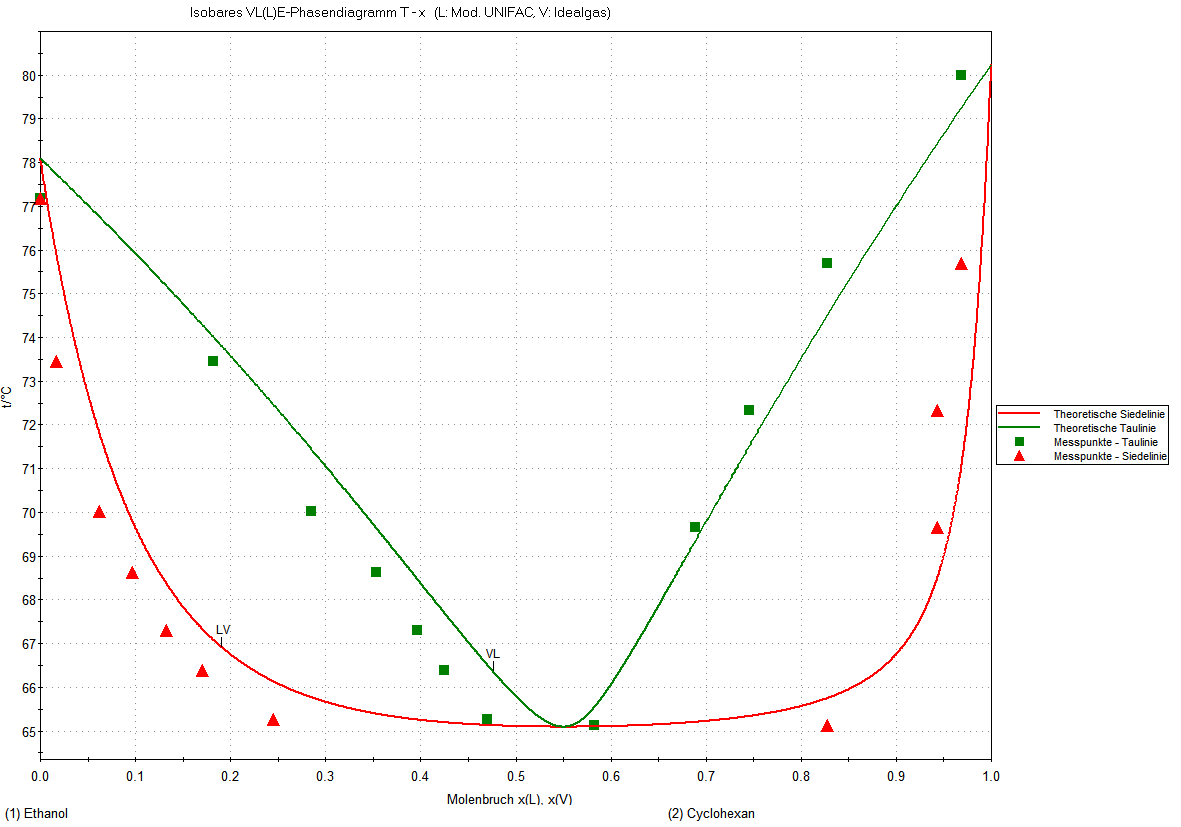
\includegraphics[width=1.1\linewidth]{img/VLE-T-x-isobar}
	\caption{Isobares Siede-/Tau-Diagramm}
	\label{fig:T-x2-isobar}
\end{figure}
Das isobare Siede-/Tau-Diagramm in Abb. \ref{fig:T-x2-isobar} zeigt auf, dass die berechneten Werte im Verlauf der theoretischen Siede- und Taulinie sehr nahe kommen. Es fallen keine offensichtlichen Ausreißer auf. Daher kann auch der, durch den Schnittpunkt der theoretischen Linien aufgezeigte, azeotrope Punkt als bestätigt angesehen werden. Dieser befindet sich etwa bei \SI{65}{\degreeCelsius} und $x_2^L=$0,55.
\begin{figure}[h!]
	\centering
	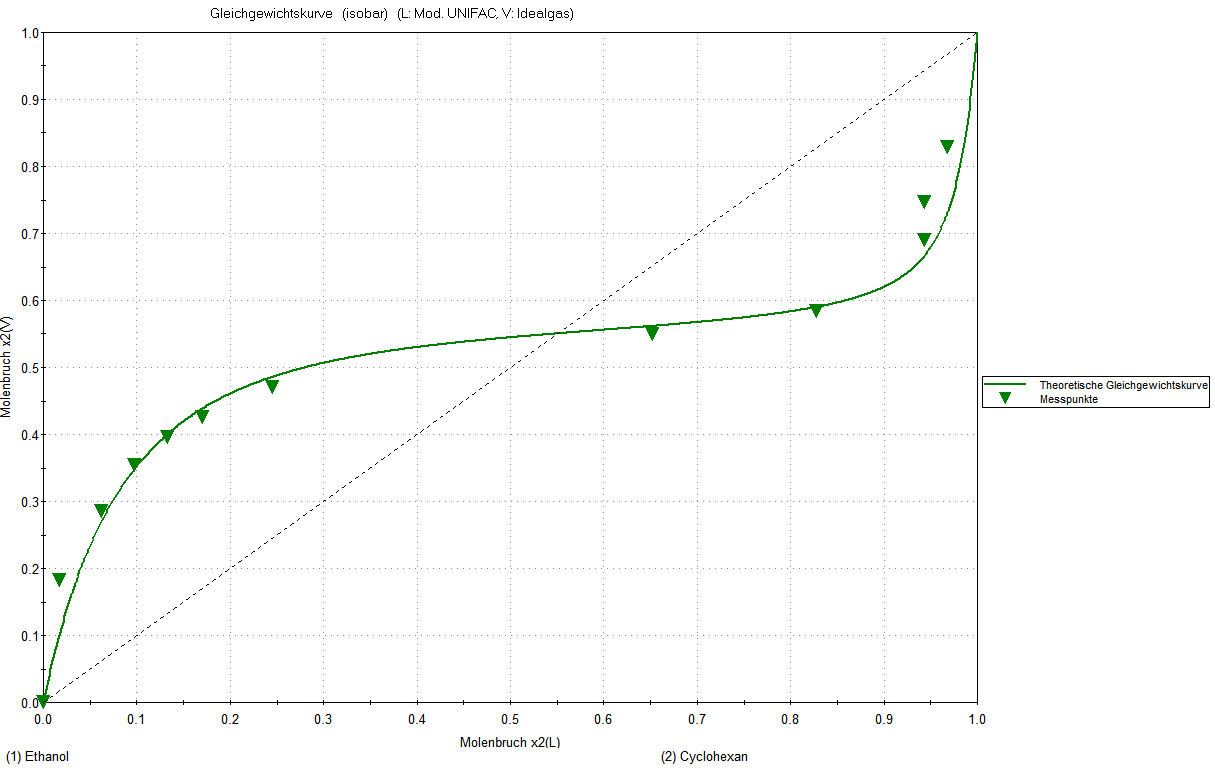
\includegraphics[width=1.1\linewidth]{img/gleichgewichtsdiagramm}
	\caption{Gleichgewichtsdiagramm}
	\label{fig:gleichgewichtsdiagramm}
\end{figure}
Das Gleichgewichtsdiagramm der Abb. \ref{fig:gleichgewichtsdiagramm} stellt den Anteil des Cyclohexans in Gas- und Flüssig-Phase gegenüber. Die Messpunkte liegen sehr nah am theoretischen Verlauf nach dem modifizierten UNIFAC-Modell. Daher sind die Messdaten als gut brauchbar zu bewerten. Der Schnittpunkt der Gleichgewichtskurve markiert wiederum den azeotropen Punkt bei $x_2^L=$0,55. Diese Erkenntnis deckt sich mit der aus dem isobaren Siede-/Tau-Diagramm.\\

\begin{figure}[h!]
	\centering
	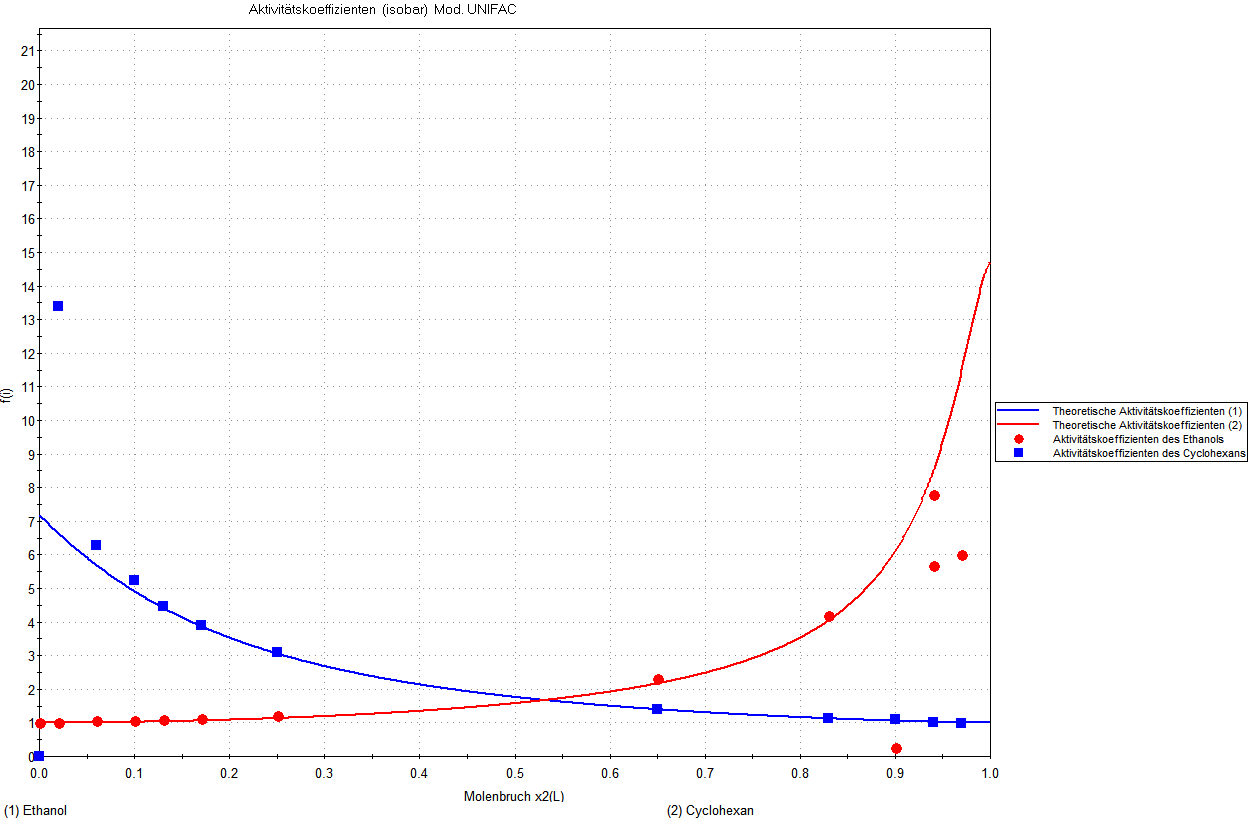
\includegraphics[width=1.1\linewidth]{img/Aktiv}
	\caption{Aktivitätskoeffizienten über dem Cyclohexananteil der flüssigen Phase}
	\label{fig:Aktiv}
\end{figure}

Die berechneten Aktivitätskoeffizienten wurden in der Abb. \ref{fig:Aktiv} graphisch aufbereitet, indem sie über dem Anteil von Cyclohexan in der Flüssig-Phase aufgetragen wurden. Auch hier stellen die durchgezogenen Linien den erwarteten Verlauf dar. In dieser Darstellung sind bereits deutliche Abweichungen zu erkennen. Da wären zum Beispiel die Aktivitätskoeffizienten des Cyclohexans am linken Rand. Der erste blaue Punkt liegt richtigerweise Im Nullpunkt des Koordinatensystems. Wenn kein Cyclohexan im System ist kann es auch keine Aktivität besitzen. Der zweite blaue Punkt könnte dafür aber als Ausreißer bezeichnet werden, wenngleich er dem vorgegebenen Trend folgt, ist er doch sehr weit von der, sonst gut angenäherten, idealen, blauen Kurve entfernt. Ähnlich verhält es sich mit den Aktivitätskoeffizienten des Ethanols bei hohen Cyclohexan-Konzentrationen. Sie folgen im allgemeinen dem Trend, weichen aber zunehmend weiter von der erwarteten Position ab. Die Aktivitätskoeffizienten weichen besonders bei niedrigen Konzentrationen von den Idealwerten ab.



\FloatBarrier










%%Tabelle START
%\vspace*{-5.5mm}
%\renewcommand{\arraystretch}{1.2}
%\begin{table}[h!]
%	\centering
%	\caption{Messwerttabelle und entsprechende Literaturwerte}
%	\label{tab:messwerttabelle}
%	%\resizebox{12.6cm}{!}{
%	\begin{tabular}{|c|c|c|c|}
%		\hline
%		\textbf{Nr.} &\textbf{p [\si{\kilo\pascal}]}	& \textbf{$\vartheta_{Messung}$ [\si{\degreeCelsius}]} &\textbf{$\vartheta_{Literatur}$ [\si{\degreeCelsius}] \cite{lideCRCHandbookChemistry1994}}	 \\
%		\hline
%		1& 100 & 81,4 & 82,2 \\
%		2& 90 & 78,8 & 79,8 \\
%		3& 80 & 76,0 & 77,2\\
%		4& 70 & 72,8 & 74,3\\
%		5& 60 & 69,2 & 71,1\\
%		6& 50 & 65,1 & 67,3\\
%		7& 40 & 60,3 & 62,8\\
%		8& 30 & 54,3 & 57,1\\
%		9& 25 & 50,6 &  53,4\\
%		10& 20 & 46,3 & 48,6\\
%		11& 10 & 33,7 & 24,1\\
%		\hline
%	\end{tabular}
%	%	}
%\end{table}
%\FloatBarrier
%\vspace*{-2.5mm}
%%Tabelle Ende
%
%In der Abb. \ref{dia:p/Tmess} sind die bestimmten Dampfdruckwerte als Funktion der Temperatur aufgetragen. Die Daten können der Tab. \ref{tab:messwerttabelle} entnommen werden.
%
%\begin{figure}[h!]
%	\begin{center}
%		%\resizebox{0.8\textwidth}{!}{
%		\begin{tikzpicture}[trim axis left, trim axis right]
%		\begin{axis}[
%		axis lines = left,
%		width = 13cm,
%		height = 7cm,
%		xmin = 0,
%		xmax = 110,
%		ymin = 0,
%		ymax = 110,
%		ytick = {0,10,...,100},
%		xtick = {0,10,...,100},
%		ylabel={Dampfdruck [\si{\kilo\pascal}]},
%		y label style={at={(-0.03,0.5)}},
%		xlabel={Temperatur [\si{\degreeCelsius}]},
%		legend style={at={(0.1,0.95)},anchor=west}
%		]
%		\addplot[black,mark=*,text mark as node=true,point meta=explicit symbolic,nodes near coords]
%		coordinates {(81.4, 100) (78.8, 90) (76, 80) (72.8, 70) (69.2, 60) (65.1, 50) (60.3,40) (54.3,30) (50.6,25) (46.3,20) (33.7,10)};
%		
%		\addplot +[mark=none, dashed, black, domain=1:100] {8570378.4523 * exp(-3215.05/(x + 201.633))};
%		
%		\addplot +[mark=+, black, domain=1:100] { 0.00000000425813333333321* x^5 + 0.000000773333333333376*x^4 + 0.0000366666666666613 *x^3 + 0.0032446667 *x^2 +1.11};
%		
%		\legend{{Isopropanol, experimentell},aus berechneter Antoine-Gleichung,{Isopropanol, Literatur}};
%		\end{axis}
%		\end{tikzpicture}
%		%	}Ventilkennlinie
%		\caption{Dampfdruckkurven}
%		\label{dia:p/Tmess}
%	\end{center}
%\end{figure}
%\FloatBarrier
%\vspace*{-5mm}
%Die Abb.\ref{dia:lnp/1/T} stellt die natürlichen Logarithmen der Damppfdrücke in \si{\kilo\pascal} als Funktion über der inversen Temperatur in Kelvin dar. Durch die Schaar der Messpunkte wurde durch lineare Regression im Tabellenkalkulationsprogramm \textsc{Libre-Office Calc} eine Trendlinie berechnet. Die Trendlinie geht auf die Funktionsgleichung (\ref{gl:Regressionsgeradengleichung}) zurück und besitzt ein Bestimmtheitsmaß von 0.99985.
%
%
%
%\subsection{Berechnung der molaren Verdampfungsenthalpie}\label{sec:berechnungMolareVerdEnthalpie}
%Die Berechnungs der molaren Verdampfungsenthalpie $\Delta_{LV}H_m$ baut auf der Clausius-Clapeyron-Gleichung auf. Es müssten folgende Annahmen getroffen werden.
%\begin{itemize}
%	\item Das molare Volumen der flüssigen Phase wird gegenüber dem molaren Volumen der Gasphase vernachlässigt.
%	\item Für den Dampf wird ideales Gasverhalten angenommen.
%\end{itemize}
%Daraus ergibt sich dann die Gleichung (\ref{gl:verdampfungsenthalpie}). Der linke Teil der Gleichung beschreibt dabei den Anstieg der zuvor ermittelten Regressionsgerade. Die Annahme idealen Gasverhaltens erlaubt auch die Verwendung der idealen Gaskonstante $R$.	\cite{molareVerdampfungsenthalpie}
%
%\begin{flalign}\label{gl:verdampfungsenthalpie}
%	\frac{d(\ln(p))}{d(1/T)}&=-\frac{\Delta_{LV}H_m}{R}\\
%	\SI{-5236,472}{\kelvin}&=-\frac{\Delta_{LV}H_m}{\SI{8,314}{\joule\per\mole\per\kelvin}}\\
%	\Delta_{LV}H_m&=\underline{\underline{\SI{43,536}{\kilo\joule\per\mole}}}
%\end{flalign}
%
%\subsection{Berechnung der Dampfdruckkurve aus den ermittelten \textit{ANTOINE}-Konstanten}\label{sec:berechnungDampfdruckkurveausKonstanten}
%
%Die ermittelten \textit{ANTOINE}-Konstanten derl Tab.\ref{tab:AntoineKonstanten} werden in die \textit{ANTOINE}\-Gleichung eingetragen. Dieser Schritt kann anhand der Gl.(\ref{gl:antoineEingesetzt}) nachvollzogen werden.
%\begin{flalign}\label{gl:antoineEingesetzt}
%	\lg(p)&=A-\frac{B}{C+\vartheta \,[\si{\degreeCelsius}]}\\
%	\lg(p)&=6,933-\frac{1396,28}{201,633+\vartheta\, [\si{\degreeCelsius}]}\\
%	p&=8570378,452304*e^{\frac{-3215,0535}{T+201,633}}
%\end{flalign}
%Die so erhaltene Dampfdruckkurve ist in die Abb.\ref{dia:p/Tmess} eingetragen. 